\documentclass{beamer}
% TODO: define things to improve class.
% TODO: slides are too similar to each other, makes readers sleepy. Replace that.


\usepackage{amssymb,amsmath}
\usepackage{graphicx}
\usepackage{url}
\usepackage{color}
\usepackage{relsize}		% For \smaller
\usepackage{url}			% For \url
\usepackage{epstopdf}	% Included EPS files automatically converted to PDF to include with pdflatex
\usepackage{pagenote}[continuous,page]

%For MindMaps
% \usepackage{tikz}%
% \usetikzlibrary{mindmap,trees,arrows}%

%%% Color Definitions %%%%%%%%%%%%%%%%%%%%%%%%%%%%%%%%%%%%%%%%%%%%%%%%%%%%%%%%%
%\definecolor{bordercol}{RGB}{40,40,40}
%\definecolor{headercol1}{RGB}{186,215,230}
%\definecolor{headercol2}{RGB}{80,80,80}
%\definecolor{headerfontcol}{RGB}{0,0,0}
%\definecolor{boxcolor}{RGB}{186,215,230}

%%% Save space in lists. Use this after the opening of the list %%%%%%%%%%%%%%%%
%\newcommand{\compresslist}{
%	\setlength{\itemsep}{1pt}
%	\setlength{\parskip}{0pt}
%	\setlength{\parsep}{0pt}
%}

%\setbeameroption{show notes on top}

% You should run 'pdflatex' TWICE, because of TOC issues.

% Rename this file.  A common temptation for first-time slide makers
% is to name it something like ``my_talk.tex'' or
% ``john_doe_talk.tex'' or even ``discrete_math_seminar_talk.tex''.
% You really won't like any of these titles the second time you give a
% talk.  Try naming your tex file something more descriptive, like
% ``riemann_hypothesis_short_proof_talk.tex''.  Even better (in case
% you recycle 99% of a talk, but still want to change a little, and
% retain copies of each), how about
% ``riemann_hypothesis_short_proof_MIT-Colloquium.2000-01-01.tex''?

\mode<presentation>
{
  % A tip: pick a theme you like first, and THEN modify the color theme, and then add math content.
  % Warsaw is the theme selected by default in Beamer's installation sample files.

  %%%%%%%%%%%%%%%%%%%%%%%%%%%% THEME
  %\usetheme{Madrid}		% No subsection
  \usetheme{AnnArbor}  % Subsection on top, no color


  %\usetheme{Antibes}
  %\usetheme{Bergen}
  %\usetheme{Berkeley}		% bem bacana - menu esquerdo
  %\usetheme{Berlin}
  %\usetheme{Boadilla}
  %\usetheme{boxes}
  %\usetheme{CambridgeUS}		% bem bacana - menu superior
  %\usetheme{Copenhagen}
  %\usetheme{Darmstadt}
  %\usetheme{default}
  %\usetheme{Dresden}
  %\usetheme{Frankfurt}
  %\usetheme{Goettingen}
  %\usetheme{Hannover}		% bem bacana - menu esquerdo
  %\usetheme{Ilmenau}
  %\usetheme{JuanLesPins}
  %\usetheme{Luebeck}
  %\usetheme{Malmoe}
  %\usetheme{Marburg}		% bem bacana - menu direito
  %\usetheme{Montpellier}
  %\usetheme{PaloAlto}		% bem bacana - menu esquerdo
  %\usetheme{Pittsburgh}
  %\usetheme{Rochester}		%bacana
  %\usetheme{Singapore}
  %\usetheme{Szeged}
  %\usetheme{Warsaw}

  %%%%%%%%%%%%%%%%%%%%%%%%%%%% COLOR THEME
  %\usecolortheme{default}		% branco, azul clarinho
  \usecolortheme{crane}		% Very yellow (ok)

  %\usecolortheme{albatross}		% azul escuro, massa
  %\usecolortheme{beetle}		% cinza, menu azul
  %\usecolortheme{dolphin}		% azul e branco, legal
  %\usecolortheme{dove}			% cinza e branco, feio
  %\usecolortheme{fly}			% todo cinza, horrível
  %\usecolortheme{lily}			% parece o default
  %\usecolortheme{orchid}		% azul e branco, ok
  %\usecolortheme{rose}			% branco e violeta-claro, bonito
  %\usecolortheme{seagull}		% cinza, feio
  %\usecolortheme{seahorse}		% nhé, meio feio
  %\usecolortheme{sidebartab}		% Azul, branco, destaque na tab, interessante
  %\usecolortheme{structure}		% bichado
  %\usecolortheme{whale}		% Azul e branco, bem bonito

  %%%%%%%%%%%%%%%%%%%%%%%%%%%% OUTER THEME
  \useoutertheme{default}
  %\useoutertheme{infolines}
  %\useoutertheme{miniframes}
  %\useoutertheme{shadow}
  %\useoutertheme{sidebar}
  %\useoutertheme{smoothbars}
  %\useoutertheme{smoothtree}
  %\useoutertheme{split}
  %\useoutertheme{tree}

  %%%%%%%%%%%%%%%%%%%%%%%%%%%% INNER THEME
  \useinnertheme{circles}
  %\useinnertheme{default}
  %\useinnertheme{inmargin}
  %\useinnertheme{rectangles}
  %\useinnertheme{rounded}

  %%%%%%%%%%%%%%%%%%%%%%%%%%%%%%%%%%%

  \setbeamercovered{invisible} % or whatever (possibly just delete it)
  % To change behavior of \uncover from graying out to totally
  % invisible, can change \setbeamercovered to invisible instead of
  % transparent. apparently there are also 'dynamic' modes that make
  % the amount of graying depend on how long it'll take until the
  % thing is uncovered.

}


% Get rid of nav bar
\beamertemplatenavigationsymbolsempty

% Use short top
%\usepackage[headheight=12pt,footheight=12pt]{beamerthemeboxes}
%\addheadboxtemplate{\color{black}}{
%\hskip0.5cm
%\color{white}
%\insertshortauthor \ \ \ \
%\insertframenumber \ \ \ \ \ \ \
%\insertsection \ \ \ \ \ \ \ \ \ \ \ \ \ \ \ \ \  \insertsubsection
%\hskip0.5cm}
%\addheadboxtemplate{\color{black}}{
%\color{white}
%\ \ \ \
%\insertsection
%}
%\addheadboxtemplate{\color{black}}{
%\color{white}
%\ \ \ \
%\insertsubsection
%}

% Insert frame number at bottom of the page.
% \usefoottemplate{\hfil\tiny{\color{black!90}\insertframenumber}}

%% makes the ppagenote command for figure references at the end.

\usepackage[english]{babel}
%qq\usepackage[latin1]{inputenc}
\usepackage{CJKutf8}
\usepackage{subfigure}

\usepackage{times}
\usepackage[T1]{fontenc}

\makepagenote
\renewcommand{\notenumintext}[1]{}
\newcommand{\ppagenote}[1]{\pagenote[Page \insertframenumber]{#1}}

\title[Programming Challenges]{GB20602 - Programming Challenges}
\author[Claus Aranha]{Claus Aranha\\{\footnotesize caranha@cs.tsukuba.ac.jp}}
\institute[U. Tsukuba]{University of Tsukuba, Department of Computer Sciences}


\title[]{Programming Challenges}
\subtitle[]{Week 4 - Combinatorics}
\author[Claus Aranha]{Claus Aranha\\{\footnotesize caranha\@@cs.tsukuba.ac.jp}}
\institute{College of Information Sciences}
\date{2015-05-11\\{\tiny Last updated \today}}

\begin{document}
\section{Introduction}
\subsection{Outline}

\begin{frame}
\maketitle
\end{frame}

\begin{frame}
  \frametitle{What is Combinatorics?}
  \begin{block}{}
    Combinatorics is the mathematics of counting.\\
    \hfill{\tiny Sounds easy, right?}
  \end{block}

  \begin{itemize}
  \item It begins with easy concepts: How to add or multiply groups;
  \item But in the end, it involves insight and advanced mathematics;
  \item It is very useful to simplify complex problems, and to
    estimate the size of sequences or combinations;
  \end{itemize}
\end{frame}

\begin{frame}
  \frametitle{Main definitions in combinatorics}
  {\small
  \begin{block}{Sequence}
    \begin{eqnarray*}
      S(1) &=& 1 = 1\\
      S(2) &=& 1 + 2 = 3\\
      S(3) &=& 1 + 2 + 3 = 6\\
    \end{eqnarray*}
  \end{block}}
\end{frame}

\begin{frame}
  \frametitle{Main definitions in combinatorics}
  {\small
  \begin{block}{Recurrence}
    The recursive form of a sequence:
    \begin{equation*}
      S(n) = S(n-1)+n; S(1) = 1;
    \end{equation*}
  \end{block}
  \begin{block}{Closed Form}
    The non-recursive form of a sequence:
    \begin{equation*}
      S(n) = \frac{n(n+1)}{2}
    \end{equation*}
  \end{block}
  } 

  The key in combinatoric problems is usually finding out the
  \structure{recurrence}, or the \structure{closed form} of a
  sequence.
\end{frame}

\begin{frame}
  \frametitle{Combinatorics: What is it good for?}
  \begin{itemize}
    \item Of course, some problems are simply to find the recurrence
      or the closed form of a sequence, or to find a specific value
      \structure{(eg. what is F(300)?)}
    \item But understanding recurrences is important to get an
      \alert{intuition about the size of things}. You can look at
      a computational problem and understand how big it can get.
  \end{itemize}
  \bigskip
  \begin{exampleblock}{}
    An intuition in combinatorics is essential to obtain an intuition
    in computational complexity.
  \end{exampleblock}
\end{frame}

\section{Outline}
\subsection{Re-learning how to count}

% Warm up rules before going to the serious stuff
% TODO: replace 4 shirts and 5 pants stuff, with an example about counting input.
\begin{frame}
  \frametitle{Warmup: Basic Combinatoric techniques}
  \begin{block}{}
    These basic rules are used to derive many of the most advanced
    combinatoric constructs.
  \end{block}
  \begin{block}{Product Rule}
    \emph{You have 4 shirts and 5 pants. How many different ways can
      you get dressed?}
  \end{block}
  \vfill
  {\small
  \begin{itemize}
  \item \structure{Product Rule:} We want to combine one element from
    set $A$, and one element from set $B$. There are $|A|\times|B|$
    different possibilities.
  \end{itemize}
  }
\end{frame}

\begin{frame}
  \frametitle{Warmup: Basic Combinatoric techniques}
  \begin{block}{}
    These basic rules are used to derive many of the most advanced
    combinatoric constructs.
  \end{block}
  \begin{block}{Sum Rule}
    \emph{The university restaurant has 3 types of curry, 5 types of
      noodles and 4 types of pasta. How many days does it take to eat
      one of each type of food?}
  \end{block}
  \vfill
  {\small
  \begin{itemize}
  \item \structure{Sum Rule:} We want to choose one element from
    either set $A$ or set $B$. Assuming the sets are independent,
    there are $|A|+|B|$ possibilities.
  \end{itemize}
  }
\end{frame}

\begin{frame}
  \frametitle{Warmup: Basic Combinatoric Techniques}
  \begin{block}{Intersection and Double Counting}
    \emph{15 students like chocolate. 13 students like vanilla. 5 of
      these students like both. How many students are there?
    }
  \end{block}
  \bigskip

  To combine sets that have repeated elements, we have to
  \structure{exclude} elements that have been counted twice, and
  \structure{include} elements that have been removed twice.
\end{frame}

\begin{frame}
  \frametitle{Intersection of sets (2)}

  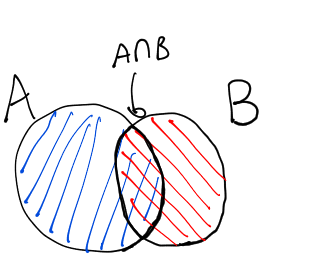
\includegraphics[height=0.4\textheight]{img/intersec1}
  \begin{block}{}
    How do we count the elements of two intersecting sets?
  \end{block}

  \begin{onlyenv}<2>
    \begin{equation*}
      |A\cup B| = |A| + |B| - |A \cap B|
    \end{equation*}
  \end{onlyenv}
\end{frame}

\begin{frame}
  \frametitle{Intersection of sets (3)}

  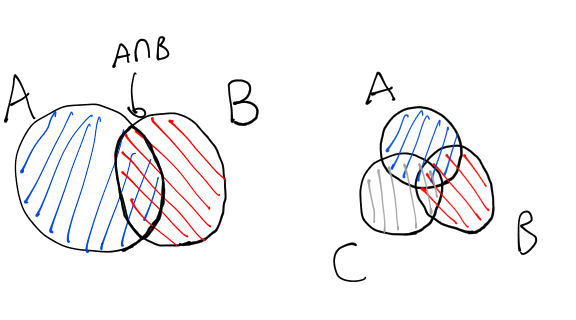
\includegraphics[height=0.4\textheight]{img/intersec2}
  \begin{block}{}
    How do we count the elements of \structure{three} intersecting sets?
  \end{block}

  \begin{onlyenv}<2>
    \begin{equation*}
      |A\cup B\cup C| = |A| + |B| - |A \cap B| + |C| - |A \cap C| - |B \cap C| + |A \cap B \cap C|
    \end{equation*}
  \end{onlyenv}
\end{frame}

\begin{frame}
  \frametitle{Intersection of sets (4)}

  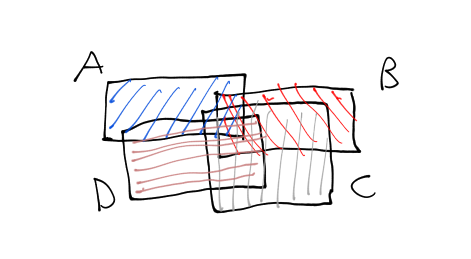
\includegraphics[height=0.4\textheight]{img/intersec3}
  \begin{block}{}
    How do we count the elements of \structure{four} intersecting sets?
  \end{block}

  \begin{onlyenv}<2>
    \begin{equation*}
      |A\cup B\cup C\cup D| = |A|+|B|+|C|+|D| - |A\cap B| - |A\cap C|
      - |A\cap D| - |B\cap C| - |B\cap D| - |C\cap D| + |A\cap B\cap
      C| + |A\cap B\cap D| + |B\cap C\cap D| - |A \cap B\cap C\cap D|
    \end{equation*}
    \bigskip
    This grows exponentially!
  \end{onlyenv}
\end{frame}

\begin{frame}
  \frametitle{What is this useful for?}
  \begin{block}{}
    Calculating set sizes is essential when estimating how fast a combination can grow!
  \end{block}
  \medskip
  {\small
  \begin{itemize}
  \item Combination sets;
  \item Problem cases -- how many possibilities for the input/output?
  \item Algorithm complexity -- how many combinations of loops?
  \item Mathematical Proofs -- proof by induction!
  \item Etc$\ldots$
  \end{itemize}
  }
\end{frame}

\section{Combinatoric Objects}
\subsection{Growth}

\begin{frame}
  \frametitle{Permutations}
  \begin{block}{Permutations}
    Arrangement of $n$ items, where every item appears exactly once:\\
    123,132,213,231,312,321
  \end{block}
  \vfill

  \begin{block}{Where do we see them?}
    \begin{itemize}
    \item Travelling salesman -- output is the permutation of cities
      in the order that they should be visited.
    \item Can you give me another example?
    \end{itemize}
  \end{block}
\end{frame}

\begin{frame}
  \frametitle{Permutations}
  \begin{block}{Permutations}
    Arrangement of $n$ items, where every item appears exactly once:\\
    123,132,213,231,312,321
  \end{block}
  \vfill

  \begin{block}{How many permutations exist for $n$?}
  \begin{itemize}
  \item<2> $n!$
    \smallskip
    
  \item<2> $3! = 6$
  \item<2> $10! = 3 628 800$
  \item<2> $20! = 2.432 +e28$
  \end{itemize}
  \end{block}
\end{frame}

\begin{frame}
  \frametitle{Subsets}
  \begin{block}{Subsets}
    A selection of $n$ items, where each item can exists or not:\\
    \{1\},\{2\},\{3\},\{1,2\},\{1,3\},\{2,3\},\{1,2,3\},\{\}
  \end{block}
  \vfill

  \begin{block}{Where do we use them?}
    \begin{itemize}
    \item The backpack problem -- Select the items that fit in the backpack.
    \item Can you give me another example?
    \end{itemize}
  \end{block}
\end{frame}

\begin{frame}
  \frametitle{Subsets}
  \begin{block}{Subsets}
    A selection of $n$ items, where each item can exists or not:\\
    \{1\},\{2\},\{3\},\{1,2\},\{1,3\},\{2,3\},\{1,2,3\},\{\}
  \end{block}
  \vfill
  \begin{block}{How many subsets are there for $n$?}
  \begin{itemize}
  \item<2> $2^n$
    \smallskip
    
  \item<2> $2^3 = 8$
  \item<2> $2^{10} = 1024$
  \item<2> $2^{20} = 1 048 576$
  \end{itemize}
  \end{block}
\end{frame}

\begin{frame}
  \frametitle{Strings}
  \begin{block}{Strings}
    A sequence of elements draw from a set \structure{with repetition}.\\
    string of length 3 from \{123\}: 222, 321, 121, ...
  \end{block}
  \vfill

  \begin{block}{Where do we see them?}    
    \begin{itemize}
    \item Game moves (e.g. Prisoner's Dilemma)
    \item Other examples?
    \end{itemize}
  \end{block}
\end{frame}

\begin{frame}
  \frametitle{Strings}
  \begin{block}{Strings}
    A sequence of elements draw from a set \structure{with repetition}.\\
    string of length 3 from \{123\}: 222, 321, 121, ...
  \end{block}
  \vfill

  \begin{block}{How fast do they grow?}
    \begin{itemize}
    \item<2> $m^n$
    \item<2> $26^5 = 11 881 376$
    \item<2> $10^{10} = 10 000 000 000$
    \end{itemize}
  \end{block}
\end{frame}

\section{Recurrence}
\subsection{Recurrence Relations}
\begin{frame}
  \frametitle{Recurrence Relations}
  \begin{block}{Definition}
    A Recurrence Relation is a function defined in terms of itself.
    \vspace{0.5cm}
    Recursion -- Recurrence -- Related words.
  \end{block}
  \begin{block}{Can you see the recursion?}
    {\small
    \begin{itemize}
      \item \structure{Tree} -- A tree has $n$ children, which can be leaf nodes or other trees
      \item \structure{List} -- \only<2>{an item links to null, or to another List}
      \item \structure{Divide-and-conquer} -- \only<2>{Divide the data, and apply the algorithm to each part}
      \item Other examples?
    \end{itemize}
    }
  \end{block}
\end{frame}

\begin{frame}
  \frametitle{Recurrence Relations}
  \begin{block}{Why are recurrences important}
    If we can find the recurrence in a sequence or in a set, we have
    found a \structure{simple algorithm} to build that sequence or
    set.
  \end{block}
  \begin{block}{}
    Recurrences are specially important for \structure{Dynamic
      Programming} (which we will talk about in a future class).
  \end{block}
\end{frame}

\begin{frame}
  \frametitle{Recurrence Relations}
  {\small
  \begin{block}{Components of a Recurrence Relation}
    \begin{itemize}
    \item Starting Condition;
    \item Recurrence Step;
    \end{itemize}
  \end{block}
  \begin{block}{Example: The Fibonacci Numbers}
    \begin{itemize}
    \item Starting Condition: $F(0) = 0; F(1) = 1;$
    \item Recurrence step: $F(n) = F(n-1) + F(n-2)$
    \end{itemize}
  \end{block}
  \begin{block}{Curiosity}
    The Fibonacci numbers were created to model the multiplication of
    rabbits.
  \end{block}
  }
\end{frame}

\begin{frame}
  \frametitle{Recurrence Relations}
  \begin{block}{}
    {\small Many functions can be easily expressed as recurrences:}
  \end{block}
  \begin{itemize}
  \item Degrees from polynomials;
    \begin{equation*}
      a_n = a_{n-1} + 1; a_1 = 1;
    \end{equation*}
  \item Exponential $(f(k,n) = k^n)$;
    \begin{equation*}
      f(k,n) = k*f(k,n-1); f(k,0) = 1;
    \end{equation*}
  \item Factorial $(f(n) = n!)$;
    \begin{equation*}
      f(n) = n*f(n-1); f(0) = 1;
    \end{equation*}
  \end{itemize}
\end{frame}

\begin{frame}
  \frametitle{Closed Form of Recurrence Relations (1)}
  \begin{block}{Definition}
    {\small
    The \structure{closed form} of a recurrence relation is a formula
    that describes the result without using the recurrence.
    }
  \end{block}
  \begin{equation*}
     F(n) = \frac{1}{\sqrt{5}}\left(\left(\frac{1+\sqrt{5}}{2}\right)^n - \left(\frac{1-\sqrt{5}}{2}\right)^n\right)
  \end{equation*}
  \vfill
  {\small
  \begin{itemize}    
  \item Closed forms are useful to quickly calculate recurrences when
    $n$ is very big;
  \item They can \structure{remove} precision errors from repeated
    multiplications;
  \item They can \structure{add} approximation errors for small $n$.
  \item Calculating closed forms is an art! (Or research topic)
  \end{itemize}}
\end{frame}

\begin{frame}
  \frametitle{Closed Form of Recurrence Relations (2)}
  {\small
  \begin{block}{Close Form for the Fibonacci Numbers}
    \begin{equation*}
      F(n) = \frac{1}{\sqrt{5}}\left(\left(\frac{1+\sqrt{5}}{2}\right)^n - \left(\frac{1-\sqrt{5}}{2}\right)^n\right)    
    \end{equation*}    
  \end{block}
  \begin{block}{We can learn things from closed forms}
    The second term of the closed form is always between 0 and 1, so
    we can calculate only the first term to estimate the value of a
    Fibonacci number;
  \end{block}
  }
\end{frame}

\section{Binomials}
\subsection{Binomials}
\begin{frame}
  \frametitle{Binomials}
  \begin{equation*}
    \binom{n}{k} = \binom{n-1}{k-1}+\binom{n-1}{k} = \frac{n!}{(n-k)!k!}
  \end{equation*}
  \begin{block}{Very important combinatory sequence}
    \structure{Basic Definition}: Number of ways you can make $k$ choices from $n$ elements.
  \end{block}
\end{frame}

\begin{frame}
  \frametitle{What can you count with binomials}
  {\small
  \begin{itemize}
    \item \structure{Probabilities}: What are the probabilities of
      your 5 numbers being chosen from the 60 in the lotto? $\frac{1}{\binom{60}{5}}$
    \item \structure{Paths Across a Grid}: How many ways are there to
      go from the top right of a $nxm$ grid to the bottom left, with the
      smallest amount of steps? $\binom{n+m}{n}$
    \item \structure{Coefficients of $(a+b)^n$}: What is the
      coefficient of $a^kb^{n-k}$? Answer: $\binom{n}{k}$. Can anyone
      explain why?
  \end{itemize}
  }
\end{frame}

\begin{frame}
  \frametitle{Computing the Binomial}
  
  \begin{block}{Closed form of the binomial}
    \begin{equation*}
      \binom{n}{k} = \frac{n!}{(n-k)!(k!)}
    \end{equation*}
  \end{block}
  \vfill
  
  \begin{itemize}
  \item What is the problem if you try to calculate that formula in a program?
  \item<2> Repeated multiplication can lead to overflow errors!
  \end{itemize}
\end{frame}

\subsection{Calculating the Binomial}
\begin{frame}
  \frametitle{Computing the Binomial}
  \begin{block}{Pascal's Triangle}
    \begin{center}
      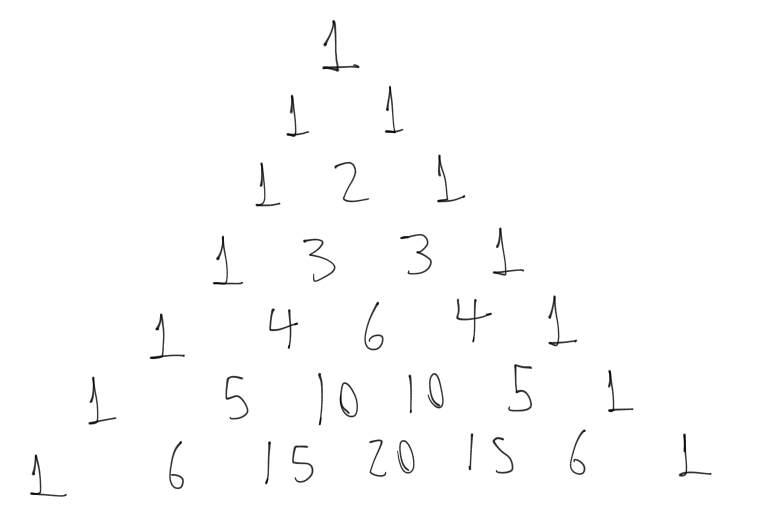
\includegraphics[height=0.7\textheight]{img/Pascal1}
    \end{center}
  \end{block}
  Have you ever played with pascal's triangle?
\end{frame}

\begin{frame}
  \frametitle{Computing the Binomial}
  \begin{block}{What can we take from pascal's triangle?}
    \begin{enumerate}
    \item Every number is the sum of its ``parents'';
    \item Every line $n$ adds up to $2^n$
    \item The numbers of line $n$ are the coefficients of $(a+b)^n$
    \end{enumerate}
  \end{block}
  \begin{block}{...wait!}
    We have seen 3 before elsewhere...
  \end{block}
\end{frame}

\begin{frame}
  \frametitle{Computing the Binomial}
  \begin{block}{Another way to see Pascal's Triangle}
    \begin{eqnarray*}
      \binom{0}{0}\\
      \binom{1}{0} \binom{1}{1}\\
      \binom{2}{0} \binom{2}{1} \binom{2}{2}\\
      \binom{3}{0} \binom{3}{1} \binom{3}{2} \binom{3}{3}
    \end{eqnarray*}
  \end{block}
  \begin{block}{}
    We know that each element of Pascal's triangle is the sum of its
    parents. This indicates that the same thing happens for binomials.
  \end{block}
\end{frame}

\begin{frame}
  \frametitle{Computing the Binomial}
  \begin{equation*}
    \binom{n}{k} = \binom{n-1}{k-1} + \binom{n-1}{k}
  \end{equation*}
  \begin{block}{}
    Let's think about the new element $n$
    \begin{itemize}
    \item What happens if $n$ is part of the sequence $k$?
    \item What happens if $n$ is NOT part of the sequence $k$?
    \item What do we do with these two sets?
    \end{itemize}
  \end{block}
\end{frame}
  
\section{Wrapping up Ideas}
\subsection{Recursion and Induction}
\begin{frame}
  \frametitle{Recursion and Induction}
  \begin{block}{}
    {\small
      Induction and Recursion are closely related to recurrence
      relations. If we can find out a correct recurrence relation for a
      combinatory construct, we can also derive a recursive algorith,
      its induction, and maybe even its closed form!
    }
  \end{block}
  \medskip
  \begin{block}{Calculating the Recursion}
    \begin{itemize}
    \item Try to figure out what the base cases are;
    \item Plot a some of the smaller values;
    \item Observe these values for patterns;
    \end{itemize}
  \end{block}

\end{frame}

\subsection{A few more Counting Sequences}

\begin{frame}
  \frametitle{Catalan Numbers}
  \begin{equation*}
    C_n = \sum_{k=0}^{n-1} C_kC_{n-1-k}=\frac{1}{n+1}\binom{2n}{n}
  \end{equation*}
  \begin{block}{}
    1,1,2,5,14,42,132,$\ldots$
  \end{block}
  \begin{block}{}
    {\small
    How many valid combinations there are for $n$ pairs of
    parenthesis? For $n = 3$, we have 5: ((())), ()(()), (())(),
    (()()) and ()()().
    \medskip
    
    Can you derive the recurrence above using this information?
    }
  \end{block}
\end{frame}

\begin{frame}
  \frametitle{Integer Partition}
  \begin{block}{}
    $f(5,5)$ = (5), (4,1), (3,2), (3,1,1), (2,2,1), (2,1,1,1), (1,1,1,1,1)
  \end{block}
  \begin{block}{}
    $f(n,k)$ Number of ways that we can sum $n$, using integers equal
    or smaller than $k$. The recurrence is $f(n,k) =
    f(n-k,k)+f(n,k-1)$, and the base cases are: $f(1,1) = 1$ and
    $f(n,k) = 0; k > n$. Can you derive this recurrence?    
  \end{block}
\end{frame}

\begin{frame}
  \frametitle{This Week's Problems}
  \begin{itemize}
  \item How Many Fibs
  \item Complete Tree Labeling
  \item Counting
  \item Steps
  \end{itemize}
\end{frame}

\begin{frame}
  \frametitle{Alert: About Week 5}
  \begin{alertblock}{Alert for Week 5!}
    There will be no class on \alert{5/18,5/22,5/25}. Week 5 only
    class will be on 5/29.
    
    \bigskip 
    
    Because of this, you will have TWO WEEKS to solve week 5's
    problems (5/16 to 5/31). The lecture notes for week 5 will be
    online this Friday.
  \end{alertblock}
\end{frame}

\end{document}
